\documentclass[../main.tex]{subfiles}

\begin{document}

\section{Overview}

This chapter describes our overall system for automatic query generation for clinical trial eligibility criteria using a natural language interface, which we call LeafAI. This system incorporates NER models (trained on the LCT corpus, described in Chapter \ref{chap:lct_corpus}), a Seq2Seq model (trained on the LLF corpus, described in Chapter \ref{chap:llf_corpus}), a KB (Chapter \ref{chap:kb}), and methods for database schema metadata tagging (Chapter \ref{chap:smm}). Section 7.2 recapitulates the motivation for our system design. Section 7.3 summarizes relevant related research described earlier in Chapter \ref{chap:background}. Section 7.4 describes methods for query generation leveraging components discussed in preceding chapters. Experimental setup and evaluation methods are described in Section 7.5, with results shown in Section 7.6. A discussion of results, implications, and limitations is presented in Section 7.7. Section 7.8 summarizes the content of this chapter.

\section{Motivation}

Identifying groups of patients meeting a given set of eligibility criteria is a critical step for recruitment into RCTs. Often, clinical studies fall short of recruitment goals, leading to time and cost overruns or challenges in ensuring adequate statistical power \cite{gul2010clinical, adams2015barriers}. Failure to recruit research subjects may result from a variety of factors, but often stems from difficulties in translating complex eligibility criteria into effective queries that can sift through data in the EHR \cite{wang2017classifying}. Despite these difficulties, RCT investigators increasingly rely on EHR data queries to identify research candidates instead of labor-intensive manual chart or case report form review \cite{cowie2017electronic}. At the same time, the amount and variety of data contained in EHRs is increasing dramatically, creating both challenges and opportunities for patient recruitment \cite{lee2017medical}. While more granular and potentially useful data are captured and stored in EHRs now than in the past, the process of accessing and leveraging that data requires technical expertise and extensive knowledge of biomedical terminologies and data models. 

Given these challenges, automated or semi-automated means of identifying eligible patients in reducing time and costs in human labor while leveraging more complex but useful data are appealing. In particular, NLP-based cohort discovery methods could be especially valuable since they can key on eligibility criteria described in natural language, a medium that clinicians, researchers and investigators already use.

\section{Related Work}

In this section we briefly summarize recent research in this domain, described earlier in Chapter \ref{chap:background}. 

Much research has explored methods for query generation, including encoder-decoder neural architectures for transforming clinical natural language questions into SQL queries \cite{bae2021question, park2021knowledge, wang2020text, pan2021bert, dhayne2021emr2vec}. The most prominent recent system and most comparable to our approach is Criteria2Query \cite{yuan2019criteria2query, fang2022combining}. Criteria2Query utilizes a combination of rule-based and neural modules to generate queries: a CRF-based NER model trained on a corpora of 230 Alzheimer's Disease eligibility criteria documents \cite{kang2017eliie}, relation extraction using Dijkstra’s algorithm \cite{chen2003dijkstra}, BERT \cite{devlin2018bert} for negation detection, Boolean logic detection using heuristics and dependency parsing, a Lucene-based \cite{lucene} OMOP mapping tool, Usagi \cite{usagi} for named entity normalization, and SuTime \cite{chang2012sutime} for temporal expression normalization. For query generation, Criteria2Query composes the resulting query representation into JSON and leverages the Observational Health Data Sciences and Informatics (OHDSI) ATLAS \cite{atlas} API to generate a SQL query.
    
\subsection{Gaps and opportunities}

Most programs capable of generating database queries do so for only a single database schema, such as OMOP or MIMIC-III \cite{johnson2016mimic}. This lack of flexibility limits their capability to accommodate real-world project needs \cite{belenkaya2021extending, peng2021towards, zoch2021adaption, warner2019hemonc, zhou2013evaluation, shin2019genomic, kwon2019development}, such as adding new database tables to OMOP for cancer staging \cite{belenkaya2021extending}. Moreover, most methods, particularly those using direct text-to-SQL deep learning approaches, tend to generate relatively simple SQL statements with few JOINs or nested sub-queries and typically no support for UNION operators and so on. This relative simplicity contrasts with the complexity of real-world EHR databases, which may contain dozens or even hundreds of tables using various vocabularies and mappings. Furthermore, direct text-to-SQL methods are bound to SQL syntax, and thus incapable of querying other systems such as Fast Healthcare Interoperability Resources (FHIR) \cite{bender2013hl7}. Additionally, few of the methods described provide support for complex logic such as nested Boolean statements or temporal sequences, and none support reasoning on non-specific criteria (e.g., "diseases that affect respiratory function"), phenomena common to study eligibility criteria \cite{wang2017classifying, ross2010analysis}. Perhaps most importantly, to the best of our knowledge, only one previous work has been tested in terms of matching patients actually enrolled in clinical trials \cite{zhang2020deepenroll}, and none have been directly compared to the capabilities of a human database programmer.

\section{Methods}

\subsection{System Architecture}

The LeafAI query engine was designed using a modular, micro service-based architecture with a central Application Program Interface (API) which orchestrates end-to-end query generation. Inter-module communication is performed using gRPC \cite{grpc}, a robust open-source remote procedure call framework which enables language-agnostic service integration. This allows individual modules to be implemented (and substituted) in programming languages and using libraries well-suited to a given task. We deploy each module as a Docker \cite{Docker} container. A diagram of the LeafAI query engine architecture is shown in Figure \ref{fig_leafai_architecture}. 

\begin{figure}[h]
  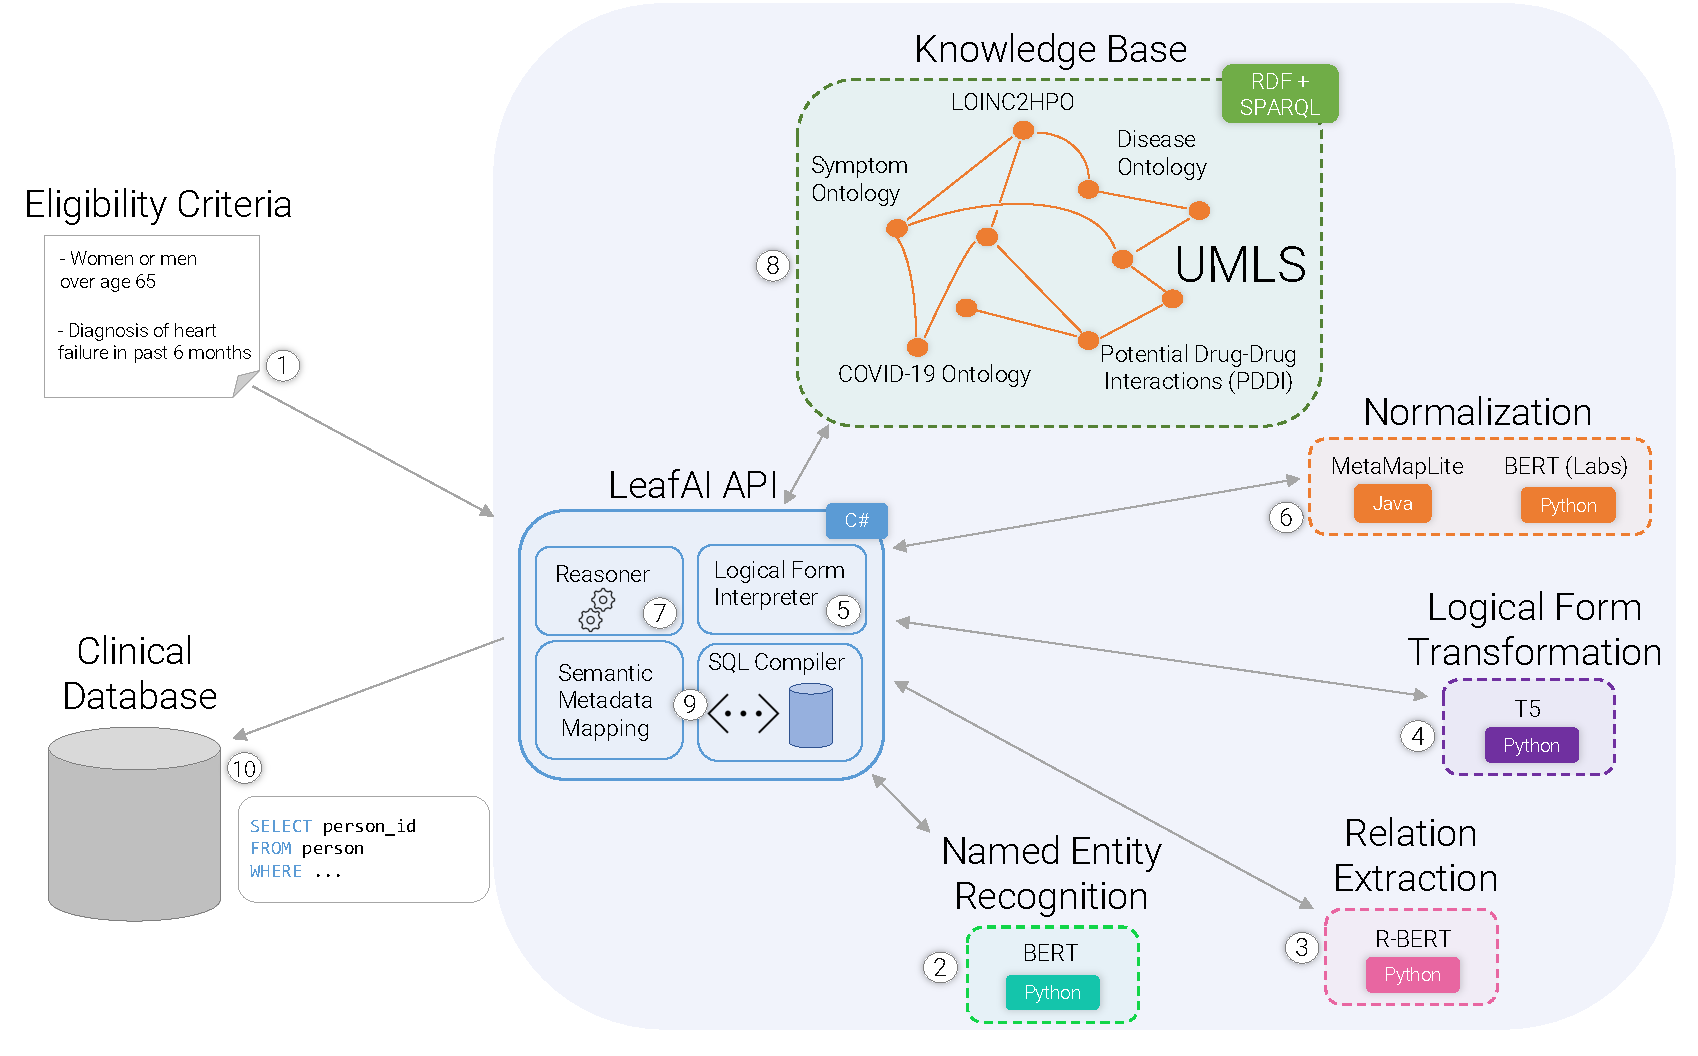
\includegraphics[scale=0.5]{Figures/7_query_generation/leafai_architecture.pdf}  
\caption{LeafAI query architecture. Inter-module communication is performed using the gRPC framework. Individual modules are deployed as Docker containers and communicate solely with the central API, which orchestrates query generation and handles query generation requests.}
\label{fig_leafai_architecture}
\end{figure}

At a high level, query generation is performed in the following steps:

\begin{enumerate}
    \item{A query request is received by the API in the form of inclusion and exclusion criteria as free-text strings.}
    \item{The input texts are tokenized and named entity recognition is performed to determine spans of text representing conditions, procedures, and so on.}
    \item{Relation extraction is performed to determine relations between the entities, such as \textit{Caused-By} or \textit{Numeric-Filter}.}
    \item{The input texts are transformed into augment text by replacing spans of "raw" text with logical form names. For example, "Diagnosed with diabetes" would become "Diagnosed with cond("diabetes")." The resulting input texts are in turn transformed into an output logical representation using a Sequence to Sequence (Seq2Seq) architecture, in the form of a string.}
    \item{A logical form interpreter module implemented as a recursive descent parser \cite{johnstone1998generalised} reads the logical form string input and instantiates it as an abstract syntax tree (AST) of nested in-memory logical form objects.}
    \item{"Named" logical form objects (i.e., specified with quoted text, such as "cond("diabetes")") are normalized into one or more corresponding UMLS concepts. UMLS child concepts are also added using our KB. For example, "cond("type 2 diabetes")” would also include concepts for type 2 diabetes with kidney complications (C2874072).}
    \item{Working recursively inside-to-outside the AST structure, each logical form object calls a \textit{Reason()} method which executes various rules depending on context.}
    \item{Each reasoning rule is performed as one or more pre-defined SPARQL queries to the KB, concept by concept.}
    \item{The final normalized, reasoned, logical form AST is thus a nested structure of UMLS concepts. Each AST criterion is mapped to zero or more corresponding entries in the semantic metadata mapping (SMM), which in turn lists meanings, roles, and relations of a database schema in the form of UMLS concepts.}
    \item{The final mapped AST object is transformed into a series of database queries, one per line of eligibility criteria text. The output SQL query can either be executed directly on a database or returned to the API caller.}
\end{enumerate}

\noindent Figure \ref{fig_leafai_querygen} illustrates an example of this process. In the following subsections we examine these steps in detail.

\begin{figure}[h]
  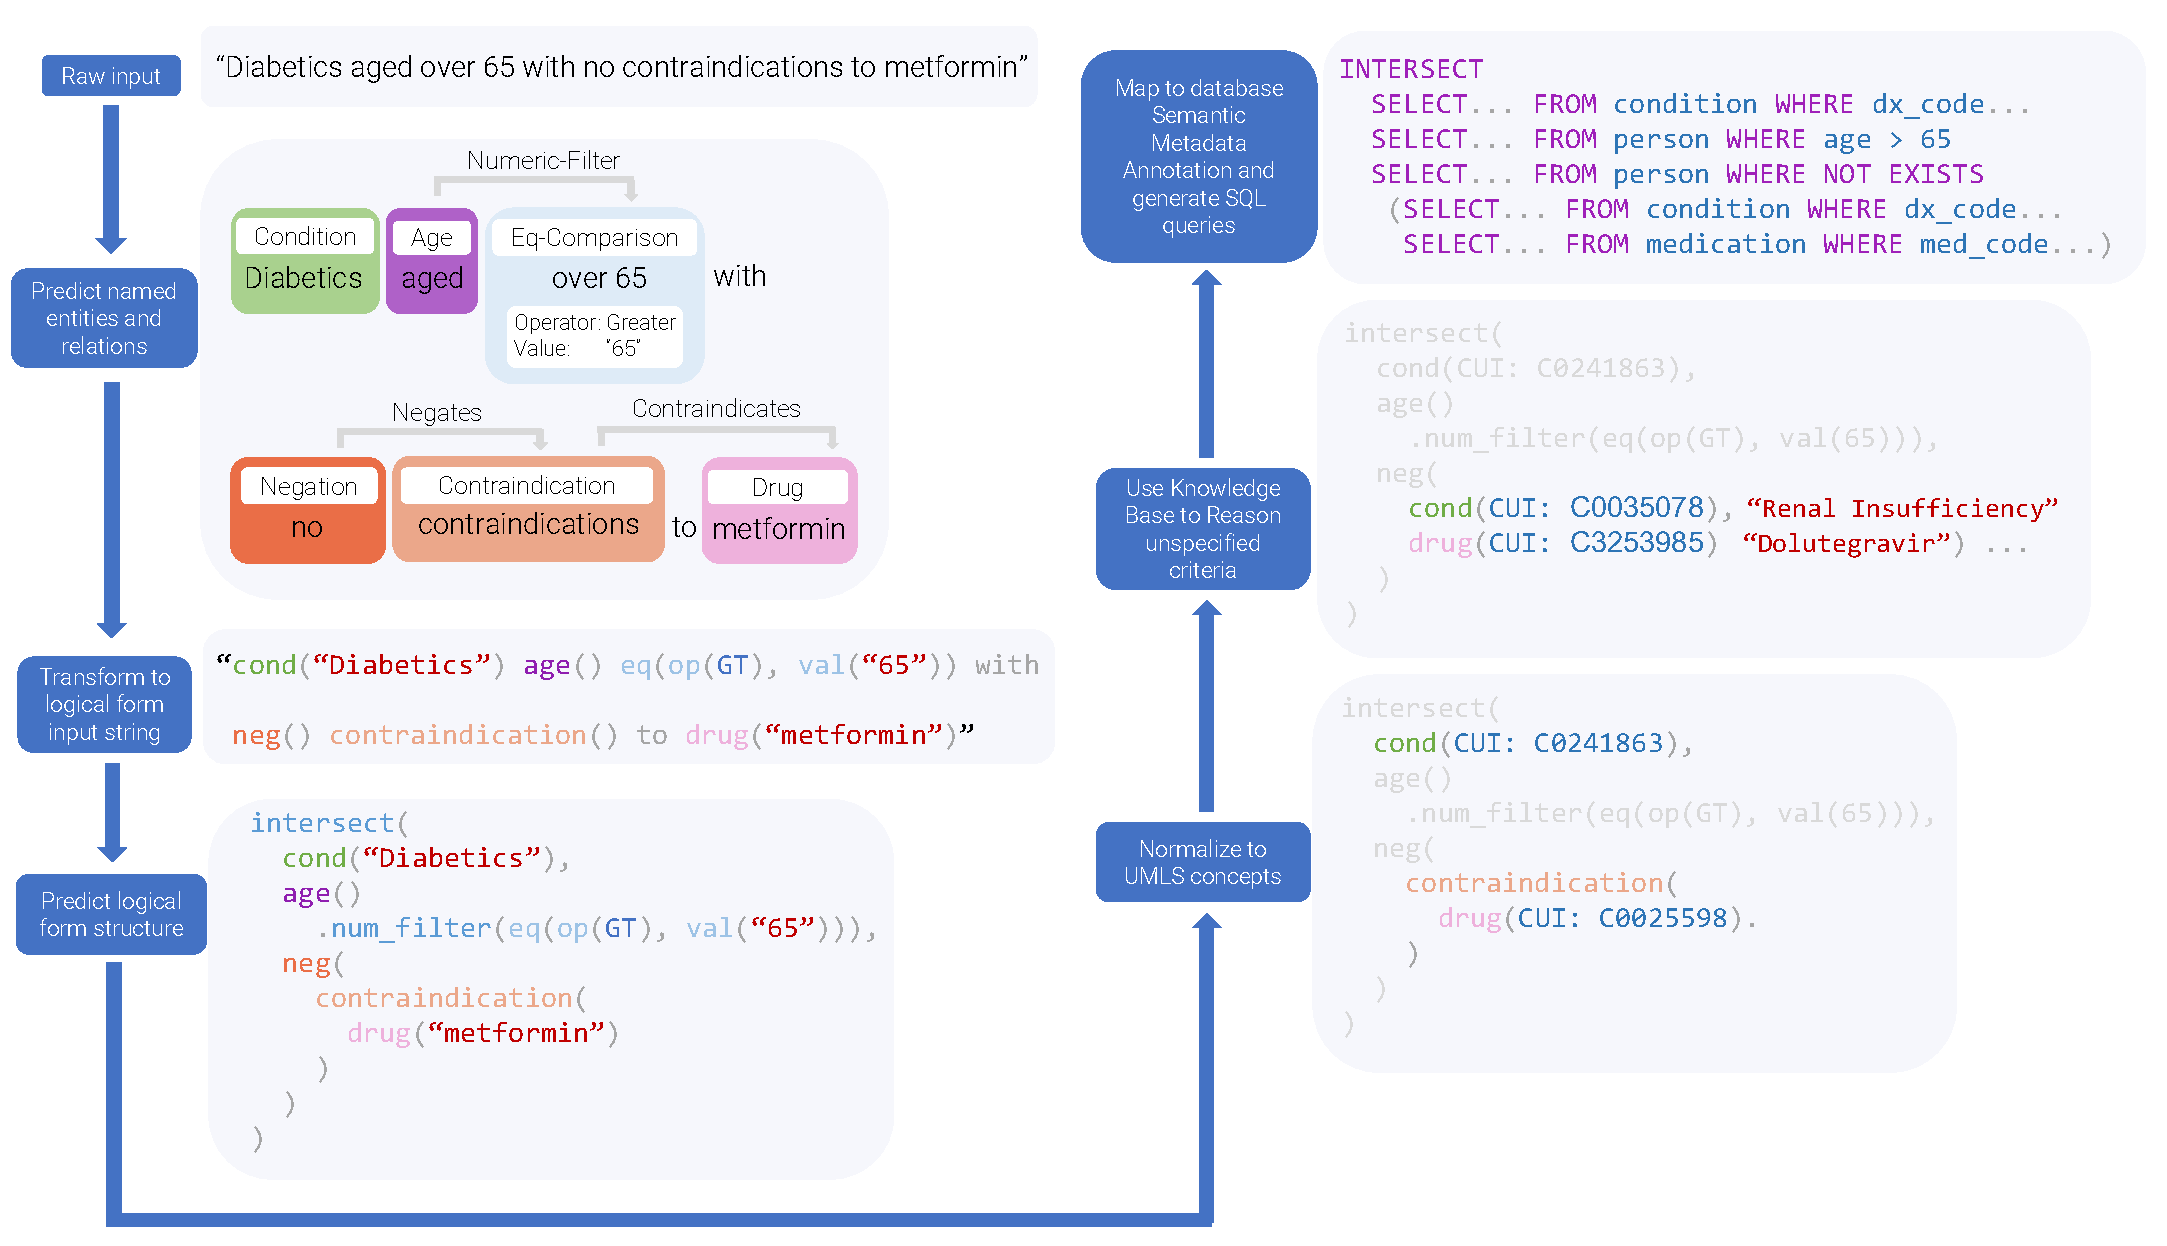
\includegraphics[scale=0.46]{Figures/7_query_generation/leafai_flow.pdf}  
\caption{LeafAI query generation processes}
\label{fig_leafai_querygen}
\end{figure}

\subsection{Named entity recognition and relation extraction}

\noindent We used the two best-performing BERT-based NER extractors from Chapter \ref{chap:lct_corpus}, one each for LCT general- and fine-grained-entities. Next, we perform relation extraction between named entity pairs similarly using a BERT-based model also trained on the LCT corpus.

\subsection{Logical form transformation}

As discussed in Chapter \ref{chap:llf_corpus}, one of the core challenges of generating queries for eligibility criteria is the problem of logical representation. Generating queries directly based on named entities and relations alone, while practical, performs poorly in cases of nested or particularly complex logic.

After NER and relation extraction are performed, we leverage our best-performing T5 Seq2Seq model fine-tuned for predicting logical forms on the LLF corpus. As inputs to the Seq2Seq model we use the original eligibility criteria with named entity spans replaced by logical form representations, as we found this improved performance compared to training with raw inputs (described in Chapter \ref{chap:llf_corpus}). For example, the criterion  

\begin{quote}
    $\textit{"Women 55 and older diagnosed with Hepatitis C"}$
\end{quote}

\noindent would be transformed to the augmented criterion

\begin{quote}
    $\textit{"female() eq(op(GTEQ), val(“55”)) diagnosed with cond(“Hepatitis C”)"}$
\end{quote}

\noindent and finally returned as the logical form

\begin{quote}
$intersect( \\
    \mathrm{\ \ \ \ }female(),\\
    \mathrm{\ \ \ \ }age().num\_filter(eq(op(GTEQ), val("55"))) \\
    \mathrm{\ \ \ \ }cond("Hepatitis\mathrm{\ }C"), \\
)$
\end{quote}

\noindent from our Seq2Seq model. The returned logical form string would then be instantiated into an abstract syntax tree (AST) of nested in-memory logical form objects using a recursive descent parser \cite{johnstone1998generalised} within our API.

\subsection{Concept normalization}

We normalize "named" logical forms to UMLS concepts using MetaMapLite \cite{aronson2001effective, demner2017metamap}, a widely used \cite{abacha2017nlm, liu2019ensembles, wang2020prediction, liu2019doc2hpo, patra2020content} and reasonably well performing rule-based application for normalization of clinical texts. We consider a logical form "named" if it contains a free-text value surrounded by quotes. For example, \textit{cond()} is unnamed and refers to any condition or disease, while \textit{cond("hypertension")} is named as it refers to a specific condition. 

Normalization using MetaMapLite can often result in high recall but low precision, as MetaMapLite has no NER component and tends to return UMLS concepts which match a given phrase syntactically but refer to abstract concepts not of interest (e.g., a search for "BMI" may return "body mass index" (C1305855), but also organic chemical "BMI 60" (C0910133)). To improve normalization precision, we employ two strategies. First, our NER component filters predicted UMLS concepts to only those of specific semantic types. For example, we limit condition concepts to only those related to semantic types of diseases or syndrome (dsyn) and so on. Next, using term-frequencies pre-computed across UMLS concept phrases, we compare term frequency-inverse document frequency (tf-idf) on MetaMapLite predictions, removing UMLS concepts whose summed matched spans have a tf-idf score lower than that of unmatched spans in a given named entity. For example, for the string "covid-19 infection", MetaMapLite predicts both "COVID-19" (C5203670) as well as several concepts related to general infections. Our tf-idf strategy removes general infection concepts because “infection” has a lower tf-idf score than the summed scores for “covid” + “-” + “19”. 

Laboratory values present a particular challenge, as LeafAI expects predicted lab concepts to have directly associated LOINC codes, while MetaMapLite typically normalizes lab test strings to UMLS concepts of semantic type "laboratory test or finding", but which do not have direct mappings to LOINC codes. For example, a search for "platelet count" returns the concept "Platelet Count Measurement" (C0032181), but not the needed concept of "Platelet \# Bld Auto" (C0362994) with LOINC code “777-3”. Thus similar to Lee and Uzuner with medications \cite{lee2020normalizing}, we trained a BERT model for sequence classification to normalize lab tests. We trained this model to identify UMLS concepts associated with LOINC codes most frequently used in eligibility criteria \cite{rafee2022elapro}, with each CUI as a possible class.

\subsection{Reasoning using an integrated knowledge base}

We leverage our KB (Chapter \ref{chap:kb}) in order to reason upon non-specific criteria using a combination of relatively simple rules within our API executed as SPARQL queries.

Our KB, nested logical forms, and inside-to-outside normalization methods enable "multi-hop" reasoning on eligibility criteria over several steps. For example, given the non-specific criterion "Contraindications to drugs for conditions which affect respiratory function", our system successfully reasons that (among other results),

\begin{enumerate}
    \item \textbf{Asthma} causes changes to \textbf{respiratory function}
    \item \textbf{Methylprednisolone} can be used to treat \textbf{asthma}
    \item \textbf{Mycosis} (fungal infection) is a contraindication to \textbf{methylprednisolone}
\end{enumerate}

\noindent These features allow LeafAI to reason upon fairly complex non-specific criteria.

\subsection{Query generation using semantic metadata mapping}

To enable data model-agnostic query generation we leverage our SMM system (Chapter \ref{chap:smm}), implemented as SQL database tables. The SMM includes metadata records of databases, tables, and columns, with corresponding foreign keys, UMLS CUI annotations, conditions, SAB encodings, and so on. The SMM is loaded from the LeafAI application database upon API startup.

\section{Evaluation}

It is reasonable to expect that an NLP-based system for finding patients based on eligibility criteria would find many  patients who actually enrolled in a real clinical trial — assuming  that patients enrolled in those trials met the necessary criteria as determined by study investigators. While there are caveats to this approach (for example, certain diagnosis codes may be missing for some patients, etc.), we suggest that tools such as LeafAI be evaluated by their ability to handle real-world eligibility criteria and clinical data. 

We compared LeafAI's results to that of a human database programmer with over 5 years of experience as a skilled analyst using SQL databases and other tools related to our EHR. Our evaluation was performed as follows:

\begin{enumerate}
    \item We extracted metadata on 168 clinical trials from our EHR between January 2017 and December 2021 where at least 10 patients were indicated as enrolled and not withdrawn, and the total number of raw lines of free-text within the eligibility criteria (besides the phrases "Inclusion Criteria" and "Exclusion Criteria") was less than or equal to 30.
    \item By manual review, we excluded 22 trials with multiple sub-groups, as it would not be possible to know which eligibility criteria applied to which sub-group of enrolled patients.
    \item To narrow the scope of our evaluation, we chose to evaluate only trials studying the following 7 disease groups: Cardiology, COVID-19, Crohn's Disease, Multiple Sclerosis (MS), Diabetes Mellitus, Hepatitis C, and Cancer. Using the "condition" field for each trial within metadata from \url{https://clinicaltrials.gov}, we filtered and grouped the remaining 146 trials into only those studying our diseases of interest. These diseases were selected to provide a diverse representation of potential queries that not only span different systems or medical specialties (infection, malignancy, cardiac, neurologic, endocrinologic) but also included conditions (COVID-19, Crohn’s disease, diabetes) commonly studied in clinical trials.
    \item We randomly chose 1 trial from each group, with the exception of Cancer, where given the large number of trials and variety of cancer types, we chose 2 trials. 427 patients were enrolled across the chosen 8 clinical trials.
    \item Both LeafAI and the human programmer were provided the raw text of eligibility criteria from \url{https://clinicaltrials.gov}, (LeafAI using API calls). Each then created queries to find patients based on each eligibility criteria, which we executed on an OMOP database derived from our EHR containing our institution’s entire research-eligible patient population.
    \item To ensure results returned would be limited to only data available during the time of each trial, we replaced references to the SQL function for generating a current timestamp (\textit{GETDATE()}) with that of each trial's end date, and similarly replaced OMOP table references with SQL views filtering data to only that existing prior to each trial's study completion date.
    \item To ensure queries would be comparable to LeafAI, the human programmer was instructed to (1) ignore criteria which cannot be computed, such as “Willing and able to participate in the study” or criteria subject to “the opinion of the investigator”, as the intents and consents of patients and investigators are unavailable in our data, (2) make a best effort to reason upon non-specific criteria (e.g., symptoms for a condition), (3) not check whether patients found by a human query enrolled within a trial, and (4) skip criteria which cause an overall query to find no eligible patients. While our team did review examples of each of these cases, we did not define formal guidelines and the human programmer instead used their best judgment.
\end{enumerate}

\section{Results}

Results of the query generation experiment are shown in Table \ref{tbl_results}. Overall, LeafAI matched 212 of 427 (49\%) total enrolled patients across 8 clinical trials compared to 180 (42\%) found by queries of the human programmer. The mean per-trial percent of patients matched was 43.5\% for LeafAI and 27.2\% for the human programmer. LeafAI had a greater number of patients determined to be eligible across all 8 trials, for a total of 27,225 eligible compared to 14,587 found by the human programmer. 

\begin{table}[h!]
    \small
    \centering
    
\documentclass[../main.tex]{subfiles}

\begin{document}

Results of our evalution are shown in Table \ref{tbl_results}.

\begin{table}[h!]
    \small
    \centering
    
\documentclass[../main.tex]{subfiles}

\begin{document}

Results of our evalution are shown in Table \ref{tbl_results}.

\begin{table}[h!]
    \small
    \centering
    
\documentclass[../main.tex]{subfiles}

\begin{document}

Results of our evalution are shown in Table \ref{tbl_results}.

\begin{table}[h!]
    \small
    \centering
    \input{tables/results}
    \caption{}
    \label{tbl_results}
\end{table} 

\begin{figure}[h!]
  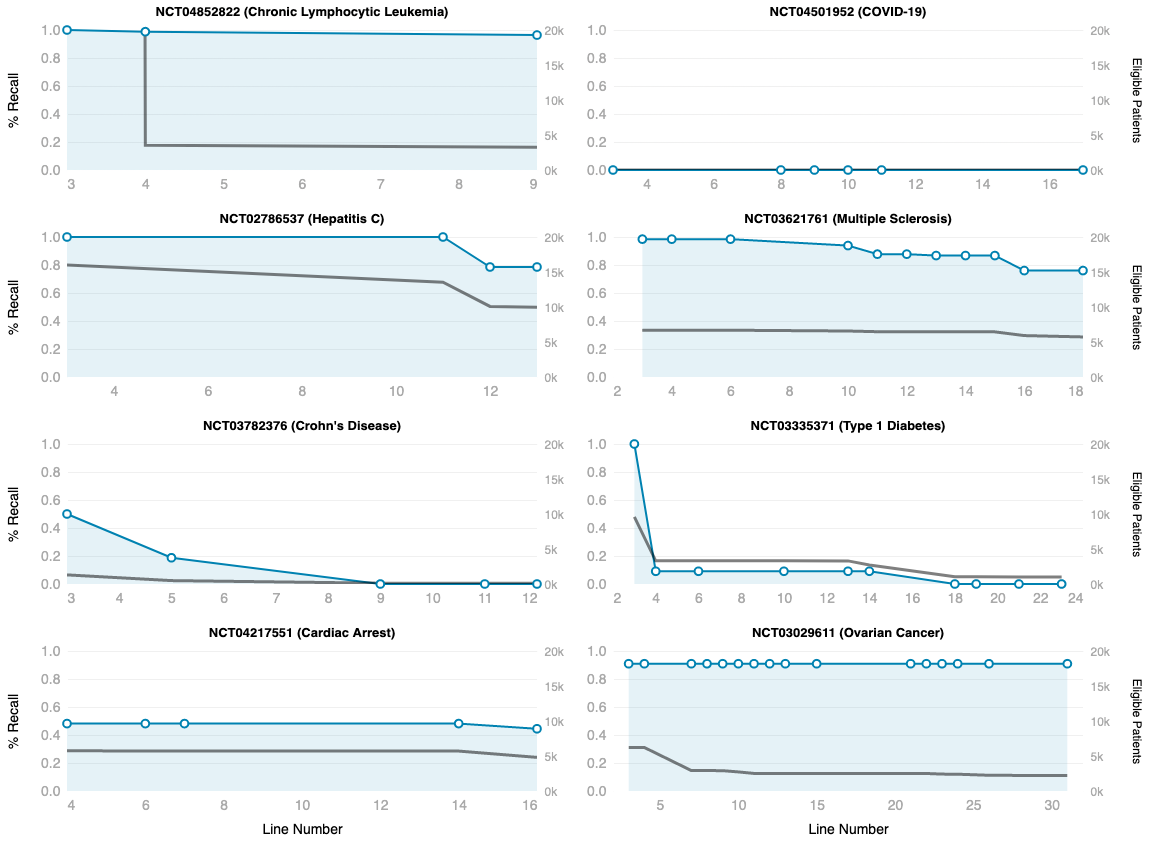
\includegraphics[scale=0.42]{figures/leafai_detail_results_longitudinal.png}  
\caption{}
\label{fig_leafai_results_longitudinal}
\end{figure}

\begin{table}[h!]
    \small
    \centering
    \input{tables/results_leafai_detail}
    \caption{}
    \label{tbl_results_leafai_detail}
\end{table} 


\end{document}
    \caption{}
    \label{tbl_results}
\end{table} 

\begin{figure}[h!]
  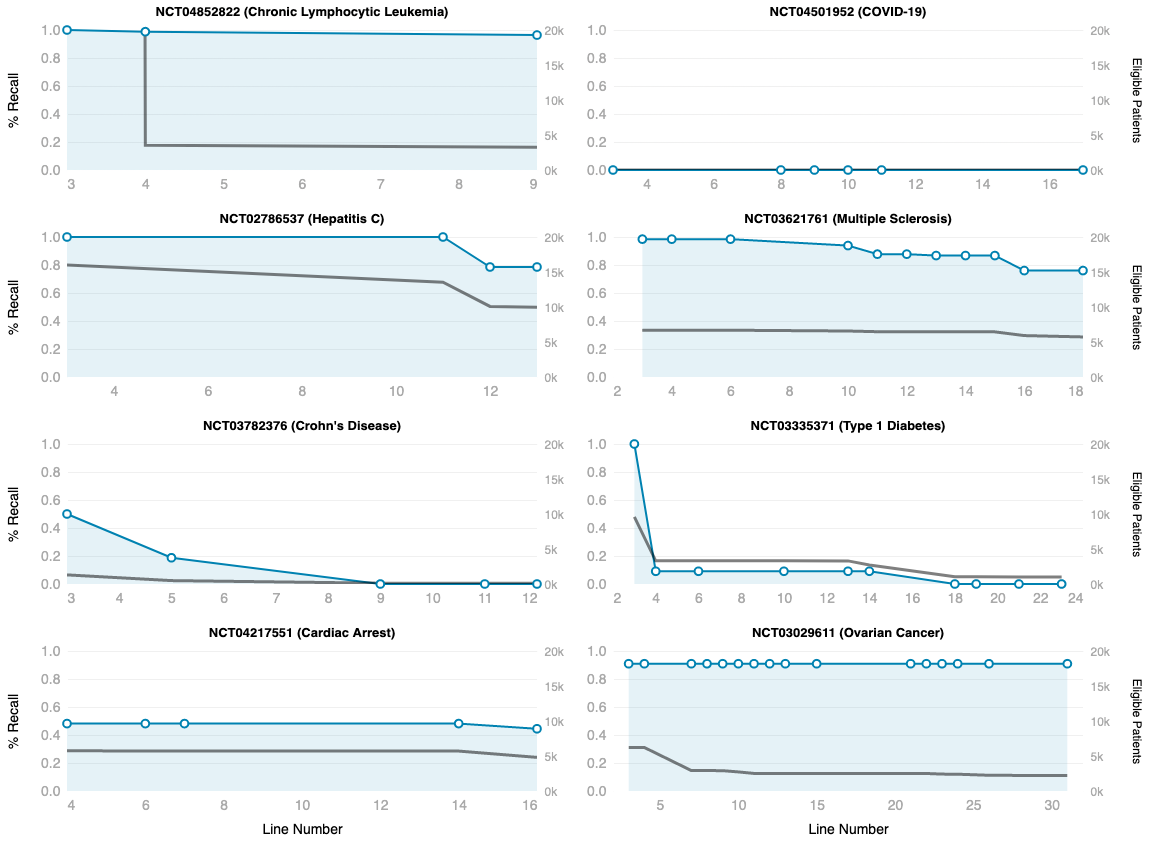
\includegraphics[scale=0.42]{figures/leafai_detail_results_longitudinal.png}  
\caption{}
\label{fig_leafai_results_longitudinal}
\end{figure}

\begin{table}[h!]
    \small
    \centering
    \def\arraystretch{1.4}
\begin{tabular}{l c c c c}
    \textbf{Condition} & \textbf{\# Criteria} & \textbf{Skipped - \newline No Patients} & \textbf{Skipped - \newline Not Computable} & \textbf{Fully Executed} \\
    \toprule
    Cl Lymphoma        & 4  & 0 (0\%)    & 0 (0\%)    & 4  (100\%)  \\
    Hepatitis C        & 8  & 0 (0\%)    & 4 (50\%)   & 4  (50\%)   \\
    Crohn's Disease    & 9  & 0 (0\%)    & 4 (44.4\%) & 5  (55.5\%) \\
    Cardiac Arrest     & 12 & 0 (0\%)    & 8 (66.6\%) & 4  (33.3\%) \\
    COVID-19           & 13 & 0 (0\%)    & 6 (46.1\%) & 7  (53.8\%) \\
    Multiple Sclerosis & 14 & 1 (7.1\%)  & 3 (21.4\%) & 10 (71.4\%) \\
    Type 1 Diabetes    & 18 & 2 (11.1\%) & 8 (44.4)   & 8  (44.4\%) \\
    Ovarian Cancer     & 25 & 2 (8\%)    & 9 (36\%)   & 14 (56\%)   \\
    \bottomrule
    \textbf{Total} & 103 & 5 (4.8\%) & 42 (40.7\%) & 61 (59.3\%)
\end{tabular}
    \caption{}
    \label{tbl_results_leafai_detail}
\end{table} 


\end{document}
    \caption{}
    \label{tbl_results}
\end{table} 

\begin{figure}[h!]
  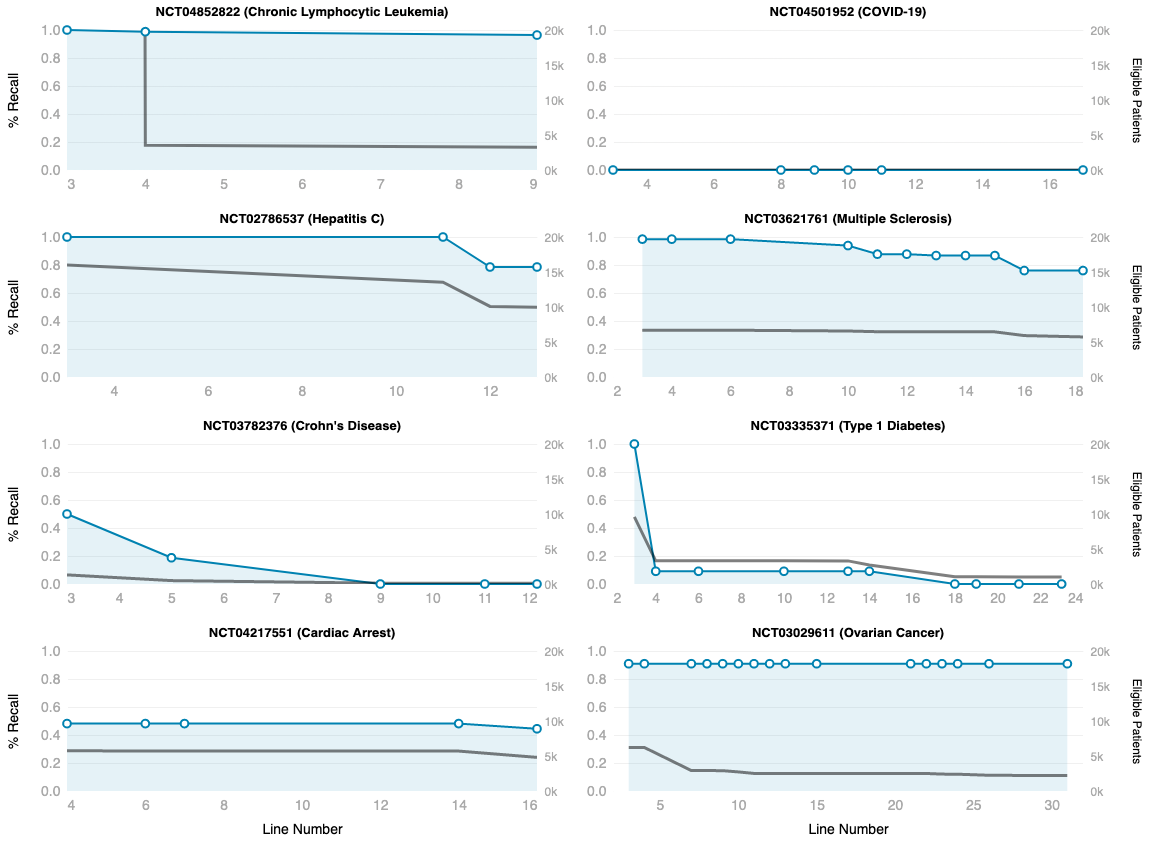
\includegraphics[scale=0.42]{figures/leafai_detail_results_longitudinal.png}  
\caption{}
\label{fig_leafai_results_longitudinal}
\end{figure}

\begin{table}[h!]
    \small
    \centering
    \def\arraystretch{1.4}
\begin{tabular}{l c c c c}
    \textbf{Condition} & \textbf{\# Criteria} & \textbf{Skipped - \newline No Patients} & \textbf{Skipped - \newline Not Computable} & \textbf{Fully Executed} \\
    \toprule
    Cl Lymphoma        & 4  & 0 (0\%)    & 0 (0\%)    & 4  (100\%)  \\
    Hepatitis C        & 8  & 0 (0\%)    & 4 (50\%)   & 4  (50\%)   \\
    Crohn's Disease    & 9  & 0 (0\%)    & 4 (44.4\%) & 5  (55.5\%) \\
    Cardiac Arrest     & 12 & 0 (0\%)    & 8 (66.6\%) & 4  (33.3\%) \\
    COVID-19           & 13 & 0 (0\%)    & 6 (46.1\%) & 7  (53.8\%) \\
    Multiple Sclerosis & 14 & 1 (7.1\%)  & 3 (21.4\%) & 10 (71.4\%) \\
    Type 1 Diabetes    & 18 & 2 (11.1\%) & 8 (44.4)   & 8  (44.4\%) \\
    Ovarian Cancer     & 25 & 2 (8\%)    & 9 (36\%)   & 14 (56\%)   \\
    \bottomrule
    \textbf{Total} & 103 & 5 (4.8\%) & 42 (40.7\%) & 61 (59.3\%)
\end{tabular}
    \caption{}
    \label{tbl_results_leafai_detail}
\end{table} 


\end{document}
    \caption{Statistics for each clinical trial evaluated by the LeafAI query engine and human programmer. The number of enrolled and matched patients were determined by cross-matching enrollments listed within our EHR. \textit{\# Crit.} indicates the number of lines of potential criteria, defined as any text besides blank spaces and the phrases “Inclusion criteria” and “Exclusion criteria”.}
    \label{tbl_results}
\end{table} 

Table \ref{tbl_results_leafai_detail} shows the number of criteria which were skipped by LeafAI. Of the 103 total criteria across all 8 studies, LeafAI executed queries for 61 (59.3\%) and skipped 5 (4.8\%) as it found no patients and 42 (40.7\%) because no computable concepts were found. 

\begin{table}[h!]
    \footnotesize
    \centering
    \def\arraystretch{1.4}
\begin{tabular}{l c c c c c}
    \textbf{Condition} & \textbf{\# Criteria} & \textbf{\# No Patients} & \textbf{\# Not Computable} & \textbf{\# Fully Executed} \\
    \toprule
    Cl Lymphoma        & 4  & 0 (0\%)    & 0 (0\%)    & 4  (100\%)  \\
    Hepatitis C        & 8  & 0 (0\%)    & 4 (50\%)   & 4  (50\%)   \\
    Crohn's Disease    & 9  & 0 (0\%)    & 4 (44.4\%) & 5  (55.5\%) \\
    Cardiac Arrest     & 12 & 0 (0\%)    & 8 (66.6\%) & 4  (33.3\%) \\
    COVID-19           & 13 & 0 (0\%)    & 6 (46.1\%) & 7  (53.8\%) \\
    Multiple Sclerosis & 14 & 1 (7.1\%)  & 3 (21.4\%) & 10 (71.4\%) \\
    Type 1 Diabetes    & 18 & 2 (11.1\%) & 8 (44.4)   & 8  (44.4\%) \\
    Ovarian Cancer     & 25 & 2 (8\%)    & 9 (36\%)   & 14 (56\%)   \\
    \bottomrule
    \textbf{Total}     & 103 & 5 (4.8\%) & 42 (40.7\%) & 61 (59.3\%)
\end{tabular}
    \caption{LeafAI and the human programmer’s handling of eligibility criteria for each trial. The column \textit{No Pats.} (Patients) indicates the count of criteria which would, if executed, cause no patients to be eligible. The column \textit{Not Computable} indicates the count of criteria which were non-computable, for various reasons. For both LeafAI and the human programmer these types of criteria were ignored. \textit{Exec.} refers to the count to fully executed queries.}
    \label{tbl_results_leafai_detail}
\end{table} 

Figure \ref{fig_leafai_results_analysis} shows differences in query strategies for 4 trials between LeafAI and the human programmer. 

\section{Discussion}

Our results demonstrate that LeafAI is capable of rivaling the ability of an experienced human programmer in identifying patients who are potentially eligible for  clinical trials. Indeed, in numerous cases we found LeafAI and the human programmer executing similar queries, such as for Hepatitis C (NCT04852822), Chronic Lymphocytic Leukemia (NCT04852822), MS (NCT03621761), and Diabetes Mellitus (NCT03029611), where both ultimately matched a similar number of patients. 243 unique patients were matched in total by either LeafAI or the human programmer, with 149 (61.2\%) identified by both.

One notable pattern we found is that LeafAI consistently finds a higher number of potentially eligible patients. We hypothesize that in many cases, LeafAI’s KB played a key role in this. For example, in the MS trial, LeafAI searched for 11 different SNOMED codes related to MS (including MS of the spinal cord, MS of the brain stem, acute relapsing MS, etc.), while the human programmer searched for only one, and ultimately LeafAI found nearly 5 times the number of potentially eligible patients (4,891 versus 1,016). It is possible that the human programmer had a lower rate of false positives (higher precision). However, determining this would come at the expense of manually reviewing tens of thousands of patient records to determine true eligibility and will be explored in a future analysis.  

On the other hand, in the same trial, as can be seen in Figure \ref{fig_leafai_results_analysis} (A), given the exclusion criteria: "Current shift work sleep disorder, or narcolepsy diagnosed with polysomnography and multiple sleep latency", LeafAI’s KB unnecessarily excluded otherwise eligible patients by removing those with diagnosis codes for drowsiness, snoring, etc., since within the UMLS those are child concepts of sleep disorder (C0851578). The exclusion of these patients likely resulted in an approximately 40\% drop in recall at that stage compared to the human programmer, though ultimately both achieved similar recall (LeafAI: 39\% versus Human: 35\%).

Another challenging pattern we identified is the normalization of text to coded values. In the Ovarian Cancer trial (NCT03029611), both LeafAI and the human programmer matched eligible patients until line 10, which specified “Serum creatinine $=<$ 2 or creatinine clearance $>$ 60 ml/min...”. The human programmer was unable to find a LOINC code for creatinine clearance and instead queried only for serum creatinine, finding 3 relatively rare tests which none of the enrolled patients had performed. In contrast, LeafAI normalized the serum creatinine test to LOINC code 2160-0, which 10 patients had performed. In the case of the Cardiac Arrest trial (NCT04217551), as in Figure 4 (D), in the first criterion, “Coma after resuscitation from out of hospital cardiac arrest”, LeafAI attempted to create a temporal sequence query for coma diagnoses, but failed to normalize “resuscitation” and skipped the criterion as non-computable. The human programmer searched for patients with a coma diagnosis, which no enrolled patients had. In the following criterion, “Cooled to $<$34 deg C within 240 minutes of cardiac arrest”, LeafAI searched for patients with a diagnosis of cardiac arrest, which 12 patients had. LeafAI ultimately matched 12 of 27 (44\%) versus zero for the human programmer.  

Beyond performance measured by recall, it is notable that the human programmer spent approximately 26 hours crafting queries for the 8 trials while LeafAI took only several minutes running on a single laptop. The time saved by using automated means such as LeafAI for cohort discovery may save health organizations significant time and resources.

\begin{figure}[H]
  \begin{center}
    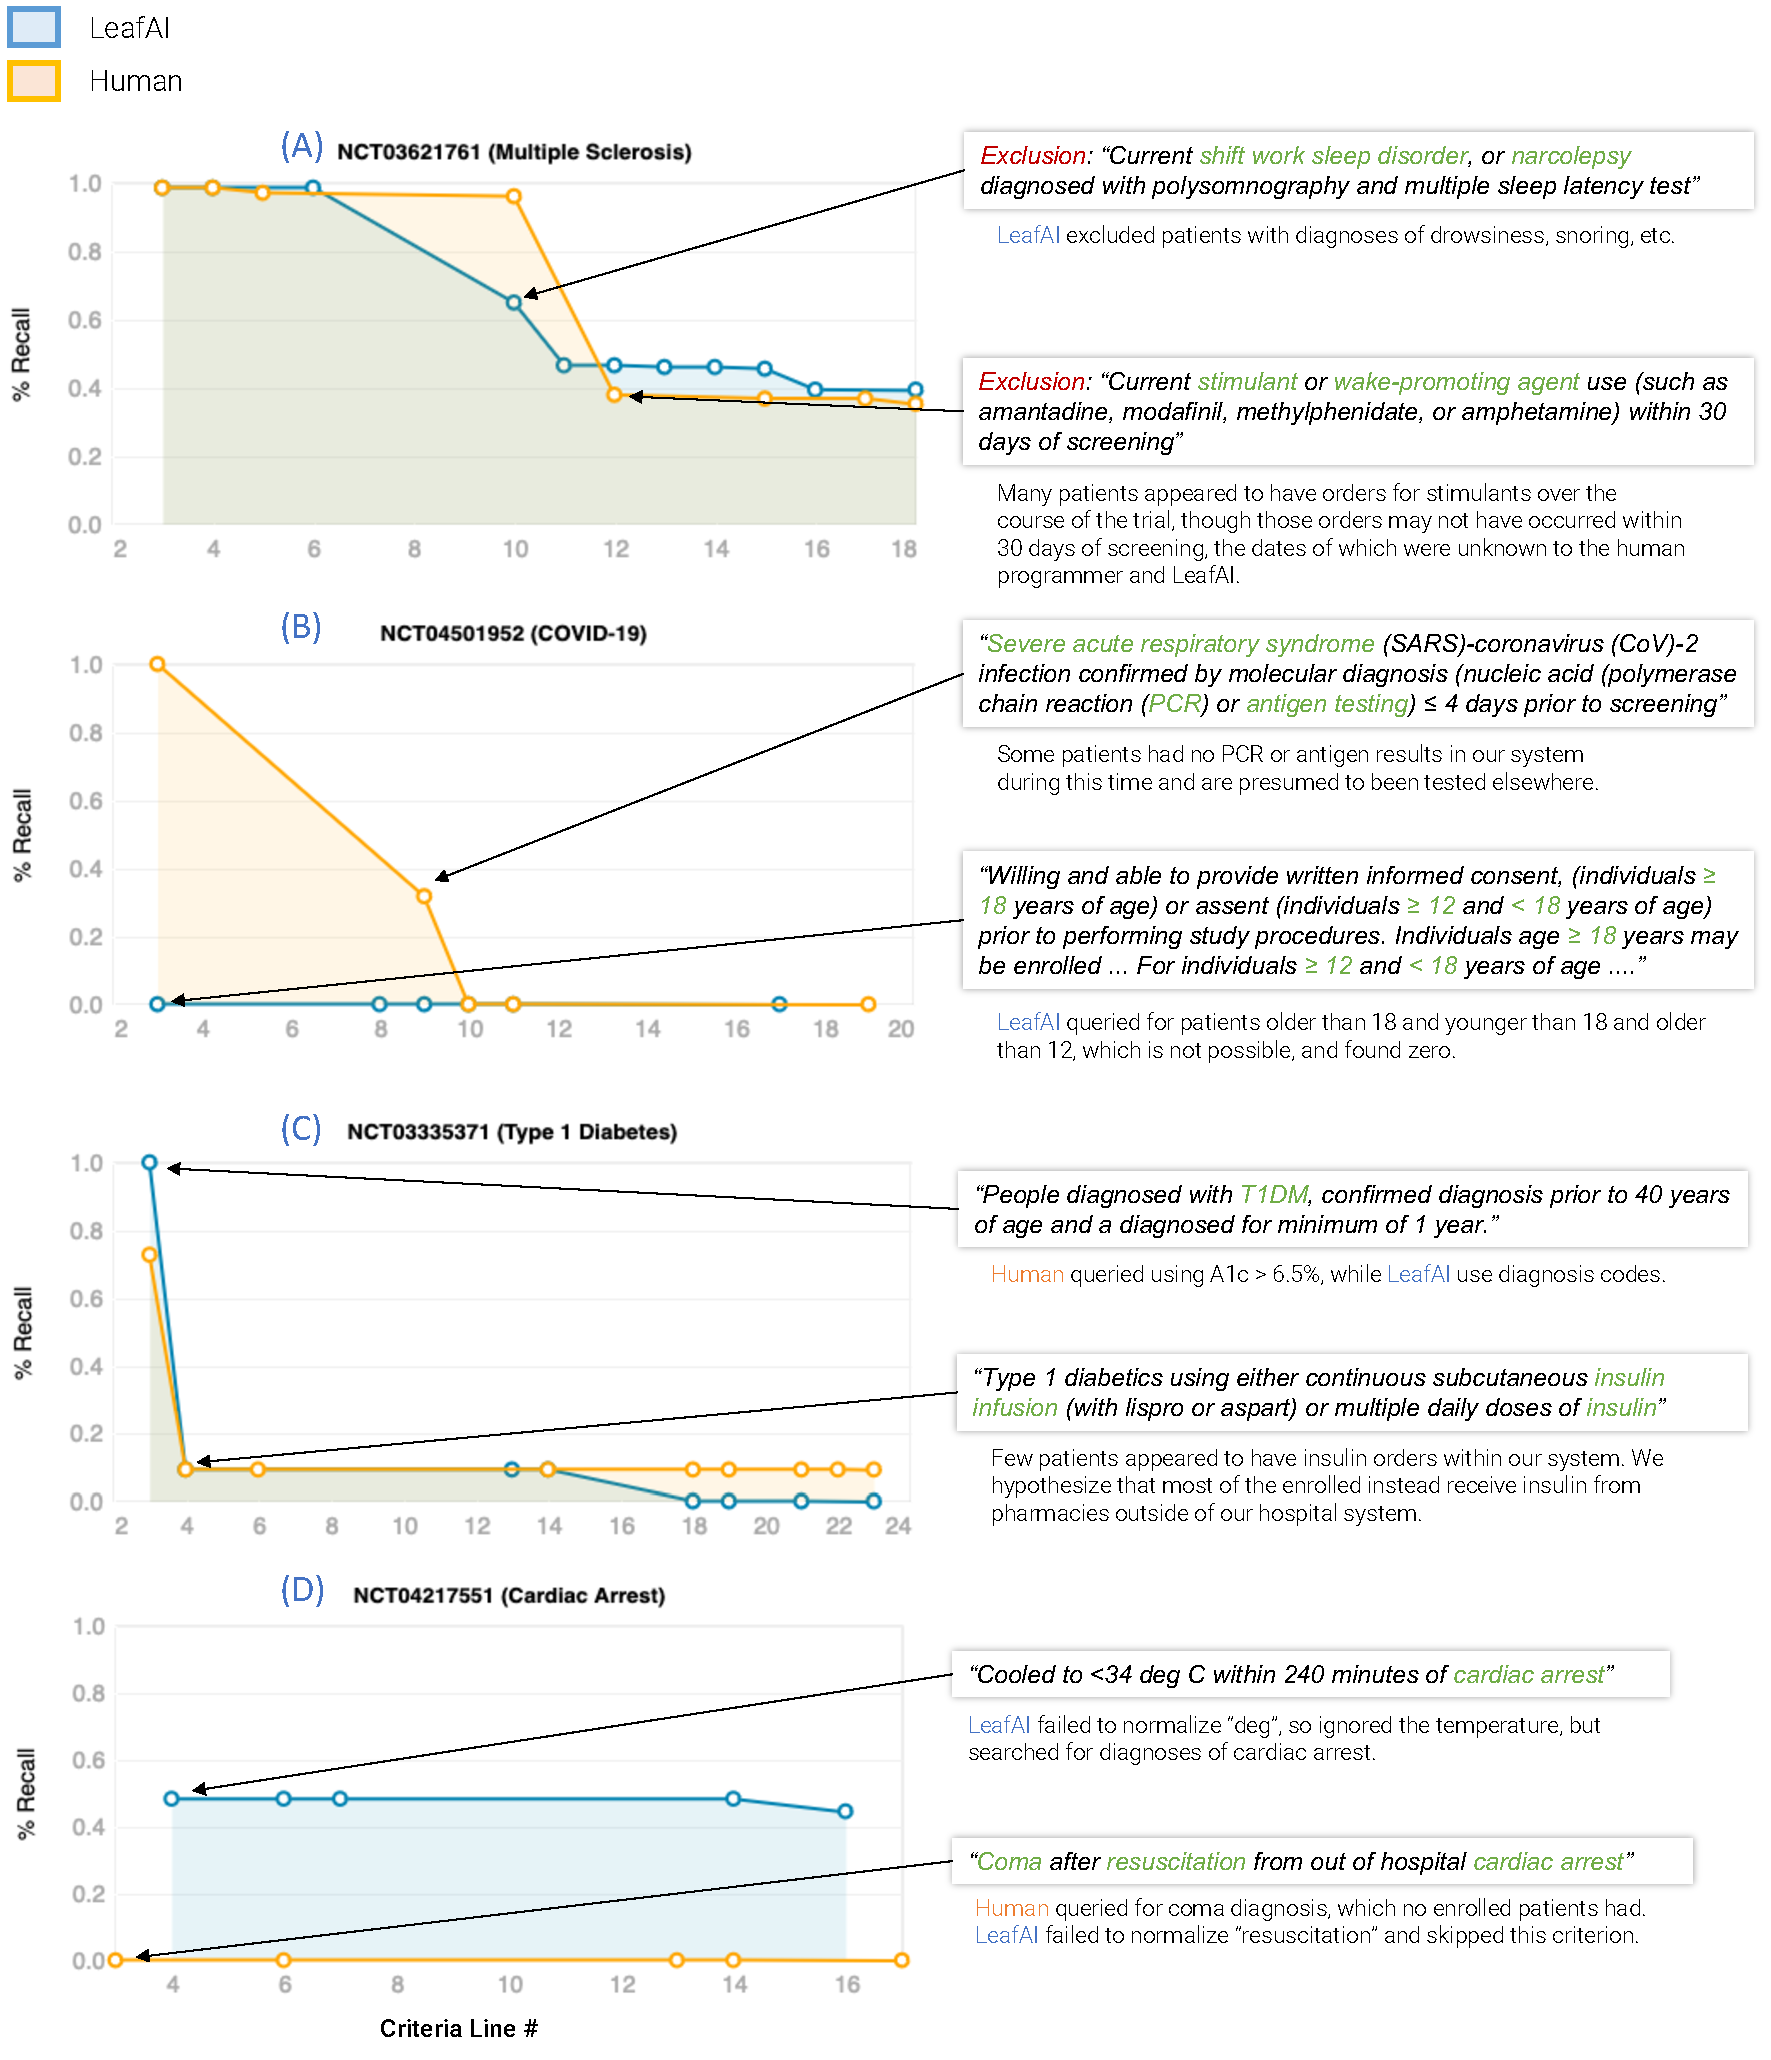
\includegraphics[scale=0.54]{Figures/7_query_generation/leafai_analysis.pdf} 
  \end{center}
  \caption{Longitudinal results for four trials. The blue line indicates recall for LeafAI and orange the human programmer. The X axis represents the line number for each eligibility criteria. Dots indicate that a query was executed for a given line. On the right, boxes represent the text of a criteria, with comments below discussing strategies and findings.}
  \label{fig_leafai_results_analysis}
\end{figure}

\subsection*{Limitations}

The LeafAI query engine and our evaluation have a number of limitations. First, while the 8 clinical trials we evaluated were randomly selected, we specifically restricted the categories of diseases from which trials were chosen and limited to trials with 30 or less lines of eligibility criteria, and thus our results may not generalize to other kinds of trials. Next, we evaluated our queries using an OMOP-based extract which did not contain the full breadth of data within our EHR. Had our experiments been conducted using our enterprise data warehouse (populated by our EHR), it is possible the human programmer would have achieved better results than LeafAI due to knowledge and experience in utilizing granular source data. For example, in the Cardiac Arrest trial, the human programmer noted that data for use of cooling blankets is available in our EHR, but not in OMOP. It is not clear how LeafAI would perform were such data available. Our tests were also limited to only one institution, and it is possible that other institutions implementing different clinical trials and accessing different databases may find different results. We also did not directly compare LeafAI to other NLP systems. While we considered comparing LeafAI to Criteria2Query \cite{yuan2019criteria2query} as part of our baseline, our analysis reviewed results longitudinally (i.e., line by line of criteria), a function which Criteria2Query does not perform. As our team members are also not expert users of Criteria2Query, any direct comparison may be biased as we may not be able to use Criteria2Query appropriately for query generation. 

Additionally, of the 103 criteria included in the 8 trials studied, LeafAI executed queries for only 56 (54\%) and the human for 52 (50\%) of them. While many criteria were unknowable (e.g., “In the opinion of investigators”) or not present in our data (e.g., “Consent to the study”), others were not computable due to failures of normalization or incorrectly predicted logical form structure. While the number of skipped criteria demonstrates that improvements to LeafAI are needed, the number of criteria found non-computable by the human programmer was similar, suggesting that potential improvements along these lines may be limited. Instead, study investigators might have to be more aware of computing shortfalls when designing criteria that will be executed by both programs and programmers; we leave a deeper analysis of this to future work. Last, the number of truly eligible patients within our institution for each trial is unknown, which impedes our ability to measure system performance. We used each trial’s known enrolled patients as our gold standard, but assume they represent only a subset of those eligible. We recognize that additional analyses regarding the false positive and true negative rates are needed. These analyses were not undertaken in this study given our limited resources and the need for manual review of many thousands of patient records to complete them.

Last, we chose to evaluate by comparing query results (i.e., returned patient IDs of those meeting criteria) rather than more traditional metrics, such as BLEU or ROUGE scores, for several reasons. First, the same query result can be returned using a variety of SQL syntax approaches, potentially unfairly penalizing a given evaluation query with a lower BLEU or ROUGE score despite returning the same query result. Second, SQL query styles can vary between human programmers as well, again potentially penalizing machine-generated approaches based on the arbitrary stylistic preferences of a given programmer used as a gold standard. More complex database schema and longer queries exacerbate both of these challenges. Last, even if these syntax and stylistic challenges were not present, we argue that the results of a query are more important regardless. One can imagine, for example, cases where a gold standard and evaluation query differ only by a single character, such as 

\begin{quote} 
\centering 
    \textit{"SELECT patient\_id FROM patients WHERE Age \textbf{$\geq$} 18"}
\end{quote}

\begin{quote} 
\centering 
    \textit{"SELECT patient\_id FROM patients WHERE Age \textbf{$<$} 18"}
\end{quote}

\noindent With the difference of only the inequality operator ($\geq$ versus $<$) the evaluation query has a relatively high BLEU score of 70.1\%, despite returning zero correct patients! Evaluating instead using the returned results would return zero patients matched and thus 0\% recall. For these reasons, we found comparison of query results rather than syntax to be a more meaningful and useful metric.

\section{Conclusions}

This chapter introduced LeafAI, a NLP-based system leveraging deep learning and an integrated KB which can automatically generate queries for cohort discovery on virtually any clinical data model. Using an OMOP database representing the entire patient population of our institution, we demonstrated that LeafAI rivals the  performance of an experienced human programmer in identifying eligible research candidates.

\end{document}